\documentclass[12pt]{article}

\usepackage[margin=1in]{geometry}
\usepackage{amsmath,amsthm,amssymb}
\usepackage{mathrsfs}
\usepackage{mathtools}
\usepackage{enumitem}
\usepackage{physics}
\usepackage{pdfpages}

\newcommand{\magsq}[1]{\big|#1\big|^2}
\newcommand{\avg}[1]{\left<#1\right>}
\newcommand{\fullint}[1][x]{\int_{-\infty}^{\infty}\dd #1\;}
\newcommand{\halfint}[1][x]{\int_{0}^{\infty}\dd #1\;}

\begin{document}
	
\title{Homework 8}
\author{Sean Ericson \\ Phys 684}
\maketitle

\section*{Problem 1}
\begin{enumerate}[label=(\alph*)]
    \item The Hamiltonian for the Lambda system in the Schr\"odinger representation is given by
    \begin{align*}
        H &= H_0 + V \\
        &= -\hbar\mqty(\omega_0&0&0\\0&0&0\\0&0&\omega_0') + \frac{\hbar}{2}\mqty(0&\Omega_0^*e^{i\omega t}&0\\\Omega_0e^{-i\omega t}&0&\Omega_0'e^{-i\omega' t}\\0&\Omega_0'^*e^{i\omega't}&0) \\
        &= \hbar\mqty(-\omega_0&\Omega_0^*e^{i\omega t}&0\\\Omega_0e^{-i\omega t}&0&\Omega_0'e^{-i\omega' t}\\0&\Omega_0'^*e^{i\omega't}&-\omega_0').
    \end{align*}
    Time evolution follows from the Schr\"odinger equation
    \begin{align*}
        \partial_t\ket{\psi} &= -\frac{i}{\hbar}H\ket{\psi} \\
        \implies& \begin{cases*}
            \dot{c}_1 =& $i\omega_0c_1 - \frac{i}{2}\Omega_0^*e^{i\omega t}$ \\
            \dot{c}_2 =& $-\frac{i}{2}\Omega_0e^{-i\omega t}c_1 - \frac{i}{2}\Omega_0'e^{i\omega't}c_3$ \\
            \dot{c}_3 =& $-\frac{i}{2}\Omega_0'^*e^{-i\omega't}c_2 i\omega_0'c_3$
        \end{cases*}
    \end{align*}
    To go to the field interaction representation, we factor out the applied field via
    \[ c_1 \to \tilde{c}_1 = c_1e^{-i\omega t}; \quad c_2 \to \tilde{c}_2 = c_2; \quad c_3 \to \tilde{c_3} = c_3e^{-i\omega't}. \]
    Then,
    \begin{align*}
        \dot{\tilde{c}}_1 &= \left(-i\omega c_1 + \dot{c}_1\right)e^{-i\omega t} \\
        &= \left(-i\omega c_1 + i\omega_0c_1 - \frac{i}{2}\Omega_0^*e^{i\omega t}\right)e^{-i\omega t} \\
        &= i\delta\tilde{c}_1 - \frac{i}{2}\Omega_0^*\tilde{c}_2 \\
        \dot{\tilde{c}}_2 &= -\frac{i}{2}\left(\Omega_0\tilde{c}_1 + \Omega_0'\tilde{c}_3\right) \\
        \dot{\tilde{c}}_3 &= \left(i\omega'c_3 + \dot{c}_3\right)e^{i\omega't} \\
        &= \left(-i\omega'c_3 + -\frac{i}{2}\Omega_0'^*e^{-i\omega't}c_2 + i\omega_0'c_3\right)e^{i\omega't} \\
        &= -\frac{i}{2}\Omega_0'^* \tilde{c}_2 + i\delta'\tilde{c}_3.
    \end{align*}
    Putting this together, we have
    \begin{alignat*}{3}
        &\quad & \partial_t \tilde{\ket{\psi}} &= i\mqty(\delta\tilde{c}_1 - \frac{1}{2}\Omega_0^*\tilde{c}_2 \\ -\frac{1}{2}\Omega_0\tilde{c}_1 - \frac{1}{2}\Omega_0'\tilde{c}_3 \\ -\frac{1}{2}\Omega_0'^*\tilde{c}_2 + \delta'\tilde{c}_3) \\
        &\quad & &= -\frac{i}{\hbar}\tilde{H}\tilde{\ket{\psi}} \\
        &\implies\quad & \tilde{H} &= \hbar\mqty(-2\delta & \frac{\Omega_0^*}{2} & 0 \\ \frac{\Omega_0}{2} & 0 & \frac{\Omega_0'}{2} \\ 0 & \frac{\Omega_0'^*}{2} & -2\delta').
    \end{alignat*}
    \item Given that
    \begin{align*}
        \ket{D} &= \frac{1}{\Omega}\left(\Omega_0'\ket{1} + \Omega_0\ket{3}\right), \\
        \ket{B} &= \frac{1}{\Omega}\left(\Omega_0^*\ket{1} - \Omega_0'^*\ket{3}\right),
    \end{align*}
    where $\Omega = \sqrt{\abs{\Omega_0}^2 + \abs{\Omega_0'}^2}$.
    The transformation between these bases is then (dropping tildes)
    \[ \mqty(c_d\\c_2\\c_B) = \mqty(\frac{\Omega_0'}{\Omega}&0&\frac{\Omega_0}{\Omega}\\0&1&0\\\frac{\Omega_0^*}{\Omega}&0&-\Omega_0'^*)\mqty(c_1\\c_2\\c_3) \eqcolon U\mqty(c_1\\c_2\\c_3). \]
    Now we can transform the Hamiltonian into this basis (assuming real Rabi frequencies):
    \begin{align*}
        H_{D2B} &= UHU^\dag \\
        &= \hbar\mqty(-2\delta & \frac{\Omega_0\Omega_0'}{\Omega^2})
    \end{align*}

    \item
\end{enumerate}


\section*{Problem 2}



\section*{Problem 3}



\section*{Problem 4}



\section*{Problem 5 (Berman 9.1-2)}

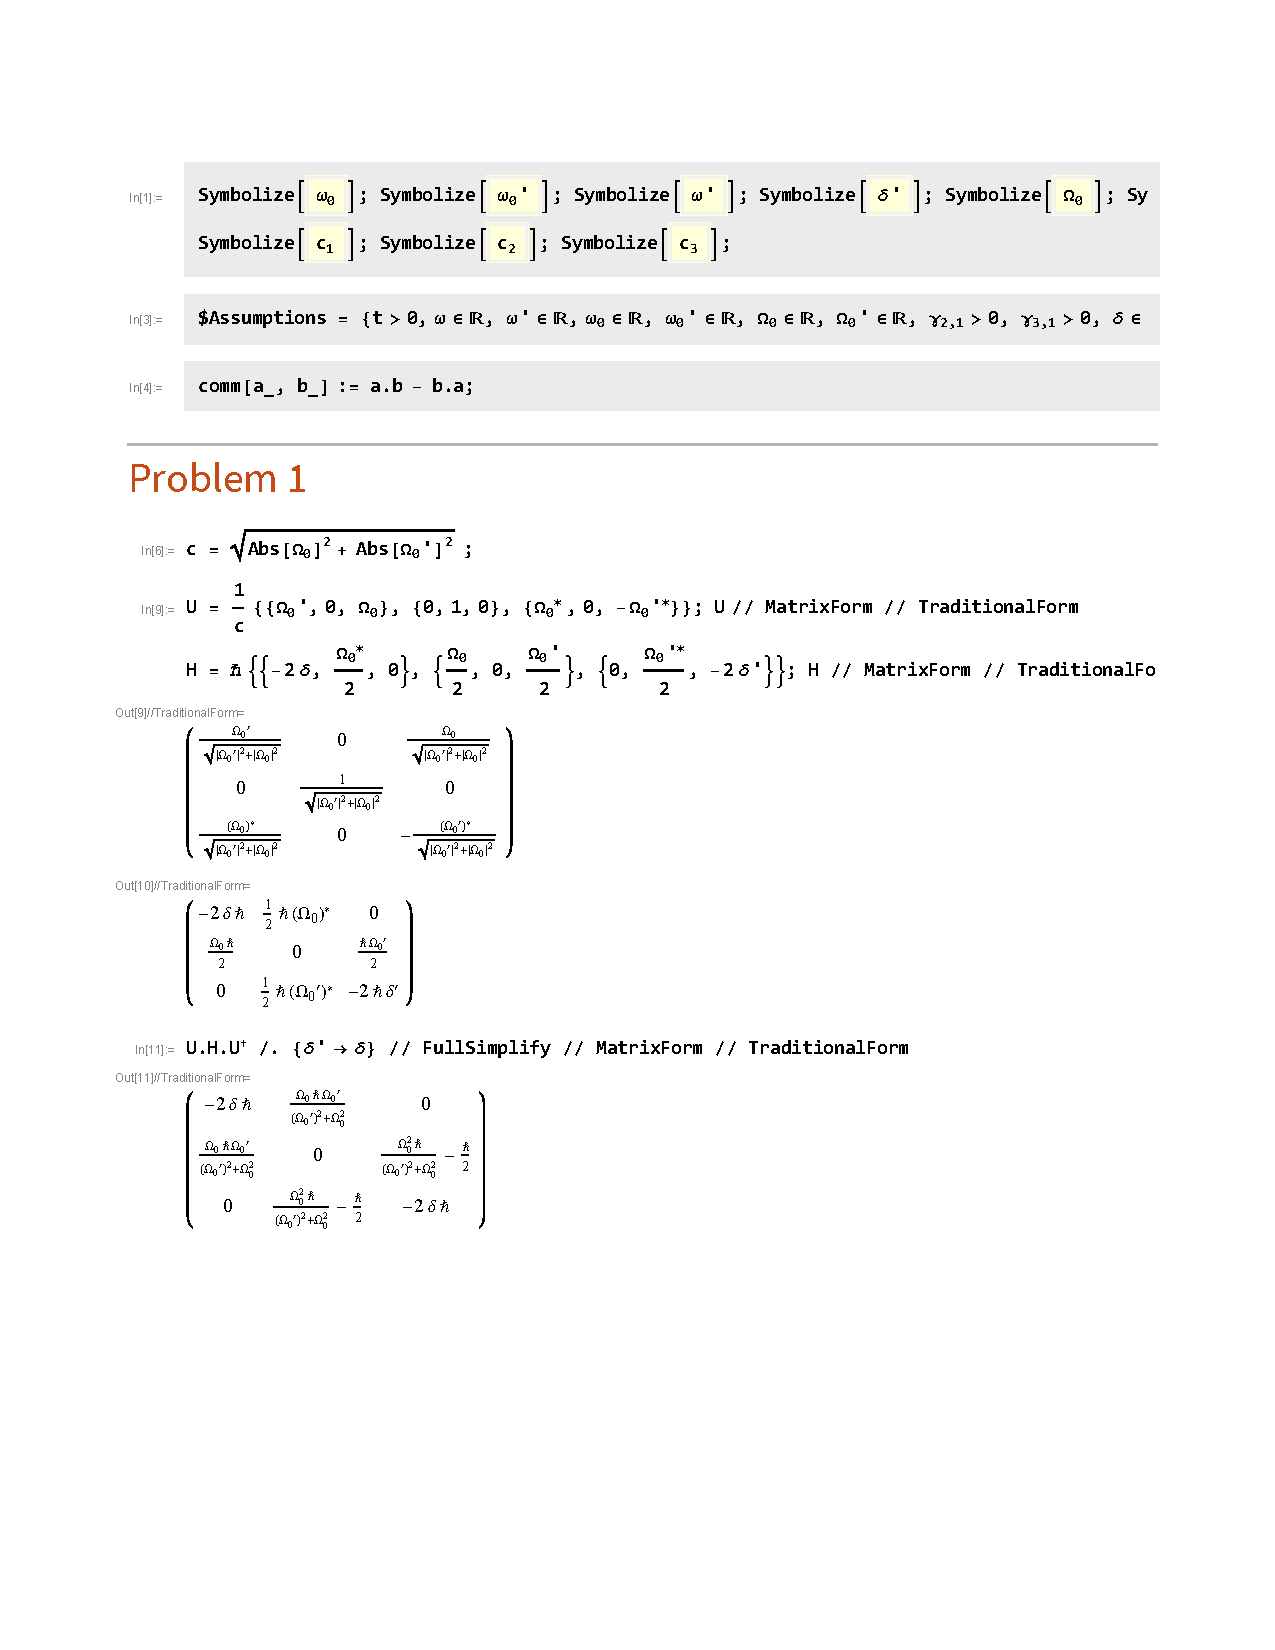
\includepdf[pages=-]{calcs/hw_8.pdf}
\end{document}